% !TeX root = ../main.tex
% Add the above to each chapter to make compiling the PDF easier in some editors.

\chapter{Einleitung}\label{chapter:introduction}
\todo{Alle Bildpositionen überprüfen!!!!}

	%Calculating the integral of a function $f(x)$ is a typical problem in numerics. In many cases, the function $f(x)$ is not known but only the function values at certain, potentially arbitrary, points. In this scenario, a common approach is to approximate the integral using the finite set of sampling points. This is a non-trivial problem.
	
	%The term \term{term} is marked like this for better understanding.
	
	%\todo{This marks a todo}{}
	Die Begriffe virtuelle Realität und erweiterte Realität kennen heutzutage viele Menschen. Allerdings wissen einige davon nicht wirklich was sich genau dahinter verbirgt. Dabei handelt es sich hierbei um zwei Forschungsbereiche, in welchen viele Firmen ein großes Potential sehen. Noch sind sie zwar unwichtig für die meisten privaten Nutzer, da die Anschaffung der bekanntesten notwendigen Geräte relativ kostspielig ist, aber In Zukunft werden diese Bereiche voraussichtlich auch dort noch weiter an Wichtigkeit gewinnen.
	Dies lässt sich bereits an den starken Entwicklungen auf dem Markt der sogenannten VR- und AR-Brillen in den letzten Jahren erkennen.
	Zwar gab es laut dem Marktforschungsunternehmen IDC einen Rückgang der Verkaufszahlen im Jahr 2018, die Prognosen für die kommenden Jahre sehen allerdings vielversprechend für diese Technologien aus, wie \refFigure{fig:forecast_diagram} zeigt \cite{verkaufVR}.
	
	\begin{figure}[htbp]
		\centering
		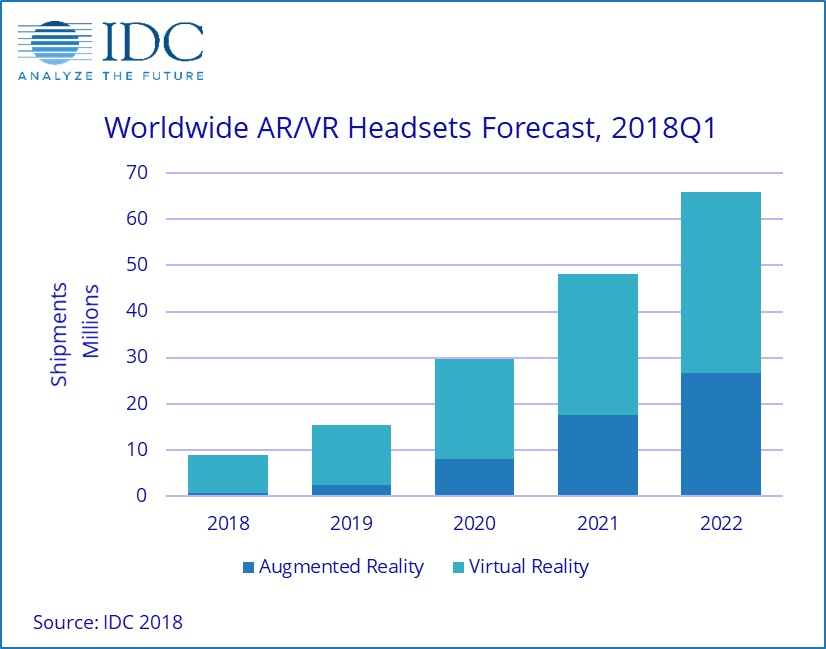
\includegraphics[width=0.6\textwidth]{figures/IDC-2018.jpg}
		\caption{Vorhersage der Verkaufszahlen nach IDC 2018 \takenFrom{verkaufVR}.}
		\label{fig:forecast_diagram}
	\end{figure}
	
	Diese speziellen Brillen dienen als Medium, um Benutzern einen Einblick in eine teilweise oder gänzlich veränderte Welt zu geben.
	Neben bereits bekannteren Exemplaren wie der HTC Vive von den Firmen HTC und Valve, der Oculus Rift von Oculus VR oder der Hololens von Microsoft, gibt es nun auch billigere Umsetzungen wie die Daydream View von Google, welche das eigene Smartphone als Display verwendet.
	Durch diese billigeren Varianten ist es auch mehr privaten Nutzern möglich ein eigenes VR-Gerät zu erwerben und auch zuhause einen Blick in virtuelle Welten zu werfen. Zudem bieten die teureren Modelle viele Möglichkeiten für die Anwendung in Unternehmen. Es wird also durch verschiedene Preiskategorien ein Angebot für jedermann erzeugt.
	%- Angebot für jedermann (durch verschiedene Preiskategorien)
	Es wird allerdings davon ausgegangen, dass die Verkäufe der Varianten von VR und AR, welche mit Hilfe von Smartphones funktionieren, durch ihre geringe Leistungsfähigkeit in Zukunft wieder zurückgehen werden \cite{verkauf2}. Für andere Modelle wird eine Steigerung der Verkaufszahlen erwartet \cite{verkaufVR}\cite{verkauf2}.
	Zudem werden weiterhin verbesserte Versionen älterer Geräte veröffentlicht. Ein Beispiel dafür ist die HTC Vive Pro, welche sowohl in der virtuellen als auch, im Gegensatz zu ihrem Vorgängermodell, in der erweiterten Realität angewendet werden kann.

	Natürlich ist die Hardwareseite nicht der einzige Punkt, an dem weitergeforscht wird. Auf der Seite der Software für diese Forschungsgebiete hat sich ebenfalls viel weiterentwickelt. Sowohl im Bereich der Unterhaltung als auch im Bereich der produktiven Nutzung, wie zum Beispiel in Form von Lernsimulationen. Allerdings sind die meisten dieser Programme nur für ein bestimmtes Gerät entwickelt worden und sind somit auf anderen Modellen nicht verwendbar. Es gibt aber auch schon einige wenige Umsetzungen von Spielen für sogenanntes \term{Crossplay} in der virtuellen Realität \cite{crossCB}. Dies bedeutet, dass diese Spiele auf mehreren Plattformen spielbar und nicht nur auf eine einzelne beschränkt sind. Bei deren genauerer Betrachtung fällt allerdings auf, dass dabei innerhalb des tatsächlichen Spiels fast komplett auf Benutzeroberflächen verzichtet wird. Somit werden zwar ein paar Schwierigkeiten umgangen, die sonst auftreten könnten, aber gleichzeitig wird das Potential von erfassten Controller- oder Handpositionen zum Anzeigen von Informationen nicht genutzt. Deshalb setzt sich diese Arbeit mit diesem Thema und möglichen Umsetzungen auseinander.
	%- Potential nicht ausgeschöpft
	%- Simulationen (Evtl Arbeit mit Drumset?)
	%- verschiedene VR Spiele und Anwendungen Screenshots!
	%- auch crossplay, aber bisher fast ohne UI
	%-Problemstellung dieser Arbeit!
	
	
	Das Ziel dieser Arbeit ist es, ein Konzept zu entwickelt, welches die Verwendung eines Programms auf mehreren Plattformen des VR- und AR-Bereichs erleichtert. Der Fokus liegt dabei auf der Platzierung der Nutzeroberfläche an verfügbaren Ankerpositionen aus der realen Welt und der Behandlung von Veränderung der Anzahl solcher Ankerpunkte.
	
	\section{Definitionen von virtueller und erweiterter Realität}
	%- Augmented Reality = Erweiterte Realität
	%- Virtual Reality = Virtuelle oder künstliche Realität
	Bei der Definition von virtueller Realität (VR) und erweiterter Realität (AR, engl. Augmented Reality) und deren Abgrenzung zueinander gibt es relativ große Meinungsunterschiede. Der Designer \term{Tidjane Tall} zum Beispiel beschreibt diese beiden Begriffe in seinem Artikel \term{Augmented Reality vs. Virtual Reality vs. Mixed Reality – An Introductory Guide} als zwei verschiedene Technologien, welche in Mixed Reality vereint werden. VR ist dabei eine Art Simulation, in der es dem Nutzer ermöglicht wird eine andere Umgebung zu sehen, als die, in der er sich tatsächlich befindet. Die erweiterte Realität hingegen definiert er durch die Projizierung computergenerierter Objekte in die reale Umgebung in Form einer Maske, welche die Realität überlagert.
	Dieses Prinzip wird beispielsweise in AR-Anwendungen für Smartphones verwendet.\cite{tidjane}
	
	Als Alternative dazu definiert \term{R. Azuma} die erweiterte Realität mit drei klaren Eigenschaften, welche den Bereich von AR weiter einschränken. Sein erster Punkt ist, dass in einem Verfahren eine Vermischung von virtuellen Bausteinen mit der Realität stattfinden müsse, damit es sich bei dessen Produkt um eine erweiterte Realität handeln kann. Um dabei allerdings Randfälle wie Bildfilter oder die simple Einblendung von Inhalten über der realen Welt auszuschließen, hat er zudem noch hinzugefügt, dass die virtuellen Elemente innerhalb der dreidimensionalen Welt platziert sein müssen. Zuletzt entfernt er noch Fälle, wie computergenerierte Inhalte innerhalb von Filmen, aus seiner Definition der erweiterten Realität, indem er nach der Möglichkeit zur Echtzeitinteraktion mit den virtuellen Inhalten verlangt.\cite{azuma}
	%-vermischung von real und virtuell
	%-Echtzeitinteraktion
	%-in der 3D Welt platziert
	
	
	%(Die virtuelle Realität (VR) und die erweiterte Realität (AR, engl. augmented reality) \todo{Checken wie das gemacht wird} bilden \todo{VR ist nicht Teilbereich sondern Grenze}) zwei Teilbereiche der Vermischung von virtueller Welt und Realität, der sogenannten Mixed Reality (MR). Bei der genauen Definition von virtueller und erweiterter Realität, sowie deren Abgrenzung voneinander, unterscheiden sich die Meinungen der ... \todo{Formulierung finden}
	
	
	Eine der verbreitetsten Definitionen stammt allerdings von \term{Milgram et al.} aus deren Arbeit \term{Augmented Reality: A class of displays on the reality-virtuality continuum}. Dabei wird der Bereich der Mixed-Reality als der Übergang zwischen der realen Welt und der virtuellen Welt definiert \cite{milgram}. Die beiden Enden zählen allerdings jeweils nicht zu diesem sogenannten Reality-Virtuality Continuum \cite{milgram}. Dieses Modell veranschaulicht \refFigure{fig:mixed_reality}. In dieser Darstellung sieht man allerdings ebenfalls, dass die erweiterte Realität innerhalb des Kontinuums nicht weiter eingegrenzt wurde, weshalb im Nachfolgenden für diesen Bereich die Definition von Azuma verwendet wird. Ansonsten gilt das Modell von \term{Milgram et al.} .
	
	\begin{figure}[htbp]
		\centering
		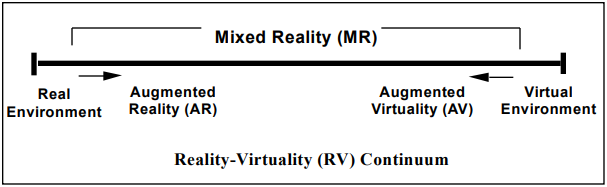
\includegraphics[width=0.75\textwidth]{figures/mixed_reality.png}
		\caption{Das Reality-Virtuality Continuum nach \term{Milgram et al.} \takenFrom{milgram}.}
		\label{fig:mixed_reality}
	\end{figure}
	
	Zur Umsetzung von VR und AR gab es in der Vergangenheit bereits mehrere Ideen, welche auf unterschiedliche Szenarien zugeschnitten sind.
	Ein Beispiel dafür ist das HUD (Head-Up Display), welches teilweise im Flugverkehr Anwendung findet \cite{azuma}.
	Die Variante mit einem HMD (Head Mounted Display) hat sich bisher allerdings in vielen Bereichen durchgesetzt, da sie durch die vollständige Kontrolle des Sehsinns ein hohes Maß an Immersion bietet und dabei nicht zwingend viel Platz verbraucht. Die Verwendung von Systemen zur Positionserkennung von Controllern, dem HMD oder von Händen in der realen Welt revidiert letzteren Vorteil aber meist wieder. Dafür kann man sich mit einem HMD relativ frei im Raum bewegen, auch wenn einige Modelle aus Gründen der Leistungsfähigkeit eine Verbindung zu einem Rechner benötigen und somit nur in der Nähe von diesem verwendet werden können. Dies ist ebenso bei der Verwendung von System zur Positionserfassung des HMDs oder der verwendeten Controller der Fall, da diese Systeme normalerweise statisch in der Welt platziert sind. Im Bereich der erweiterten Realität ist diese Bindung allerdings oft störend. Sie lebt schließlich von der realen Welt, in welcher sich der Benutzer bewegen können soll. Deshalb gibt es Bemühungen die Notwendigkeit eines stationären Computers zu beheben, ohne dabei die Performanz zu mindern. Ein Durchbruch hierbei ist die Hololens von Microsoft, welche ohne zusätzlichen Computer funktioniert. Sie hat dementsprechend aber weniger Leistung, weshalb ein kontinuierliches Erkennen der Handpositionen nur im Sichtfeld ermöglicht wird.
	%- Head Mounted Display
	%- Mischung von Realität und virtuellen Elementen
	%- AR lebt von der realen Welt und somit von freiem Bewegen
	%-> nicht an Pc gebunden
	%--> weniger Leistung
	%--> kein Handtracking

	\section{Benutzeroberflächen}
		%- Schnittstelle zwischen Nutzer und Programm
		Im Bereich der Mensch-Maschine-Interaktion, kurz HCI (Human-Computer-Interaction) wird im Groben zwischen drei Bereichen unterschieden: Mensch, Maschine und deren Schnittstelle.
		
		
		Die Benutzeroberfläche (UI, engl. User Interface) stellt eben jenen Übergang zwischen Maschine und Mensch dar und ermöglicht die Interaktion beider Seiten miteinander \cite{GUI}.
		%- nur die graphische Seite GUI betrachtet
		Sie lässt sich weiter in physische Steuerelemente und graphische Bestandteile (das GUI, engl. Graphical User Interface) aufteilen. Zu dem ersten Bereich zählen alle Arten von Knöpfen, Hebeln, Reglern und Sensoren, welche Eingaben durch den Nutzer ermöglichen, ebenso wie visuelle, haptische oder akustische Ausgabegeräte, welche dem Nutzer eine Rückmeldung zu dessen Aktionen geben und den Status des ausgeführten Programms an den Benutzer weiterleiten.
		
		
		Der graphische Anteil, der in dieser Arbeit betrachtet wird, stellt dem Nutzer über Texte, Bilder und Farben Informationen zur Verfügung und kann deren Manipulation ermöglichen. Damit soll Benutzern die Erfassung und Veränderung der virtuellen Umgebung erleichtert werden.
		Die graphische Benutzeroberfläche hat die früher übliche Kommandozeile abgelöst um die Darstellung von Informationen und Funktionen des Systems auf eine verständlichere und ansprechende Art zu ermöglichen. Sie liegt in Form einer Maske vor, welche auf einem Bildschirm angezeigt werden kann. Im Fall einer Interaktion führt sie vordefinierte Befehle aus und wird dabei gegebenenfalls verändert. Dadurch ist es nicht mehr nötig die einzelnen Befehle und deren Auswirkungen zu kennen, was die Benutzung eines Programms besonders für Neulinge erleichtert.
		%-Stellt Information zur Verfügung und ermöglicht die Erfassung und Manipulation der virtuellen Umgebung
		Die Inhalte der Oberfläche werden meist innerhalb von Menüs und Untermenüs geordnet, um sie übersichtlicher darzustellen.\cite{GUI}
	
		\subsection{Element}
			%- Beispiele: Textfeld, Bild, Schaltfläche...
			Die graphische Benutzeroberfläche setzt sich aus einzelnen Elementen zusammen. Diese können beispielsweise Texte, Bilder oder Schaltflächen sein, welche normalerweise innerhalb einer Menüstruktur untereinander oder nebeneinander angeordnet sind. Sie enthalten Informationen und Funktionen, welche durch das Auswählen des jeweiligen Elements aufgerufen werden können.
	
		\subsection{Anker}
			%- Position an welcher Elemente der Benutzeroberfläche platziert werden
			Ein Anker bezeichnet eine Position, zu welcher die Elemente der Benutzeroberfläche relativ platziert werden.
			In Desktop-Programmen werden dafür die Bildschirmkanten beziehungsweise Ecken verwendet.
			
			%-Beispiel aus Unity
			\begin{figure}[htbp]
				\centering
				\includegraphics[width=0.4\textwidth]{figures/Ui_Anchor_Unity.png}
				\caption{Anker Beispiel aus Unity\takenFrom{unity}.}
				\label{fig:unity}
			\end{figure}
			
			Am Beispiel aus der Spiel-Engine Unity (siehe \refFigure{fig:unity}), sieht man eine Auswahl an möglichen Ankerpositionen innerhalb des Anwendungsfensters. Zudem sind verschiedene Kombinationen von Verbindungen zu zwei oder mehr Ankern angegeben, wodurch eine Vergrößerung oder Verkleinerung mit dem Anwendungsfenster durchgeführt werden kann.
	
	\section{Definition der Umgebungsabhängigkeit}
		%- UI befindet sich im 3D Raum und kann von Objekten verdeckt werden. Sie ist an eine 3D Position gebunden und kann sich unabhängig vom Benutzer verschieben und rotieren, sie muss also nicht statisch zur Kamera sein
		Als umgebungsabhängig werden in dieser Arbeit Benutzeroberflächen bezeichnet, welche sich, im Gegensatz zum herkömmlichen zweidimensionalen Äquivalent, im dreidimensionalen Raum befinden und somit auch von Objekten aus der virtuellen oder realen Umgebung verdeckt werden können. Sie sind somit nicht wie eine Maske, die zwischen Kamera und der Umgebung angezeigt wird, sondern wie Bestandteile der, den Nutzer umgebenden, Welt. Zudem müssen sie sich nicht statisch zu, beziehungsweise abhängig von, der Kamera bewegen, sondern können auch an einen anderen Gegenstand aus der Umgebung gebunden werden, mit dem sie sich mitbewegen und gegebenenfalls mitrotieren. Diese Gegenstände werden in dieser Arbeit \term{Ankerobjekt} genannt.
		In 3D-Programmen (siehe \refChapter{chapter:3dPos}) wird solche UI häufig an Objekten positioniert und ist zu diesen statisch. In Spielen handelt sich dabei meist um eine diegetische Benutzeroberfläche und gilt als Teil der Umgebung \cite{diegetic}. An einem Beispiel aus \term{Metro: Last Light} (siehe \refFigure{fig:diegetic}) sieht man, wie ein zweidimensionales Textobjekt an einem Blatt Papier in der dreidimensionalen Umgebung platziert wurde.
		
		%-Beispiel aus Unity
		\begin{figure}[htbp]
			\centering
			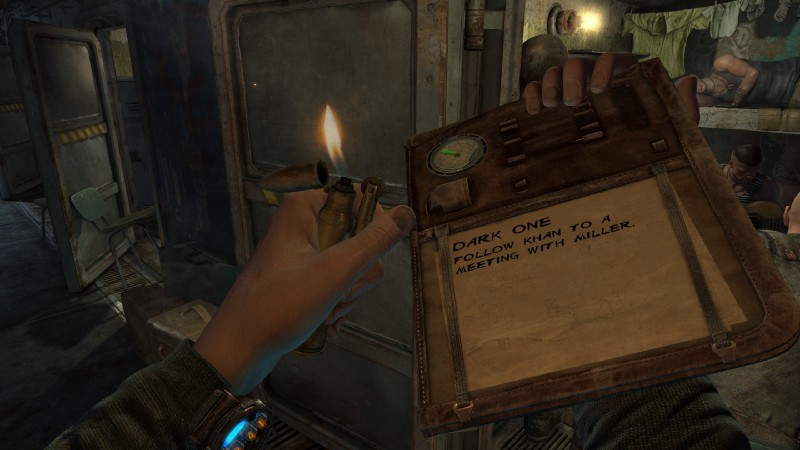
\includegraphics[width=0.7\textwidth]{figures/diegeticUI.jpeg}
			\caption{Diegetisches Element im Spiel \term{Metro: Last Light} \takenFrom{diegetic}.}
			\label{fig:diegetic}
		\end{figure}
	